\section{Mechanical Design}
\label{sec:mechanical_design}
%Decision making is like the brain of the overall system. How system react to the environmental changes and how inputs/measurements affect the system are determined in this component of the system.
%Total Maximum weight = 10 kg
%Food reservoir = 4kg
%Weight of the electronic components = 3kg 
%Feed two times.
%One meal is 31 gr
In this module, the following sections will be discussed.
\begin{itemize}
    \item Subsystem Description
    \item Tests and Results, Future Test Plans
    \item Modifications
    \item Compatibility Analysis of Mechanics
\end{itemize}

\subsection{Subsystem Description}

Mechanical design is composed of two parts namely:
\begin{itemize}
    \item Exterior design
    \item Interior design
\end{itemize}

The exterior design is composed of the outer design of the box. It should satisfy the upper conditions. The expected weight of the food reservoir and the electronic components respectively is 4 kg and 3 kg, which add up to 7 kg. An average person can lift \%15 of their body weight which corresponds to 11 kg for a 70 kg person without giving any harm to their body \cite{cite:CWH}. Therefore, an ordinary person can easily carry our system. 
The expected size of the box is 40X30 $cm^{2}$ base and 53 cm height which its volume is 63 liter. The technical drawing can be seen in Fig~\ref{fig:OuterBox}. 

%TODO: Technical resimlerin yerini düzenle
\begin{figure}[h!] %Pardon burası
     \centering
     \begin{subfigure}[b]{0.49\linewidth}
     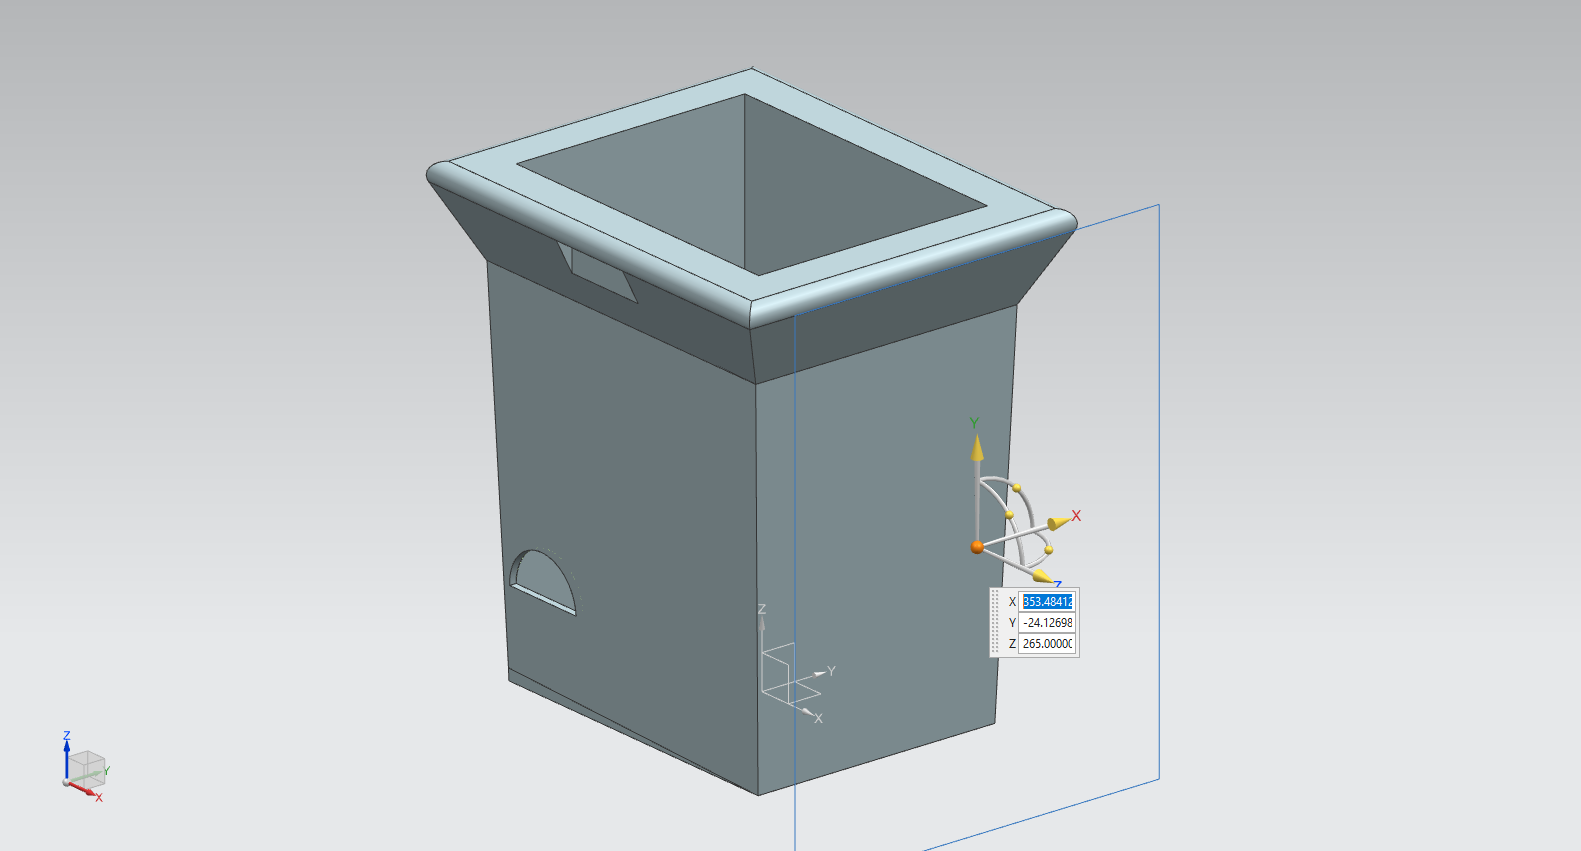
\includegraphics[width=\linewidth]{content/060_mechanical_design/3box.png}
     \end{subfigure}
     \begin{subfigure}[b]{0.49\linewidth}
     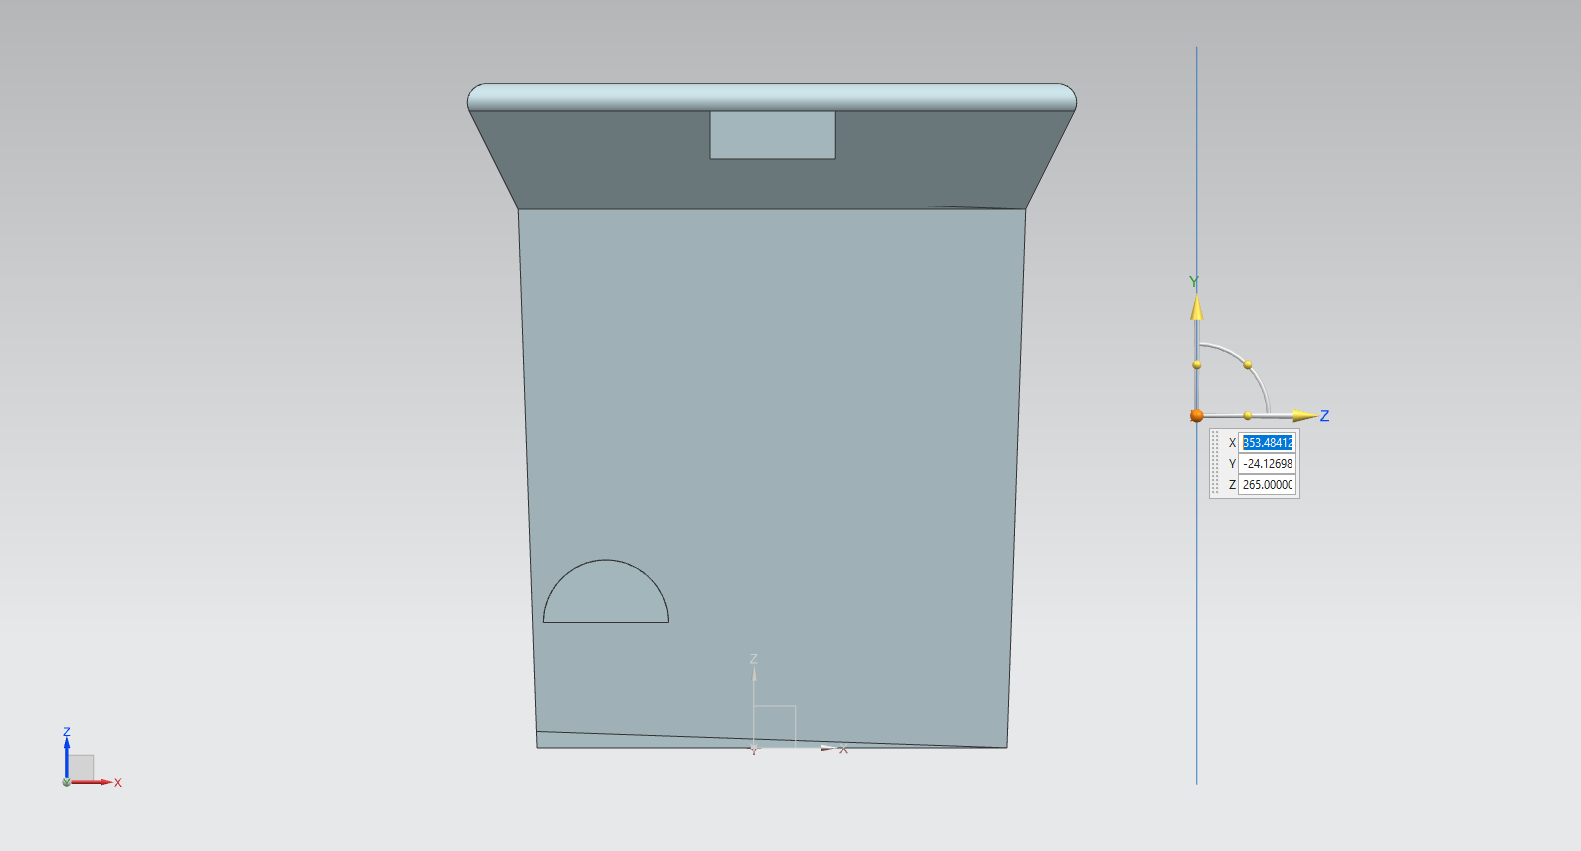
\includegraphics[width=\linewidth]{content/060_mechanical_design/4box.png}
     \end{subfigure}
     \label{fig:pwm}
     \begin{subfigure}[c]{0.49\linewidth}
     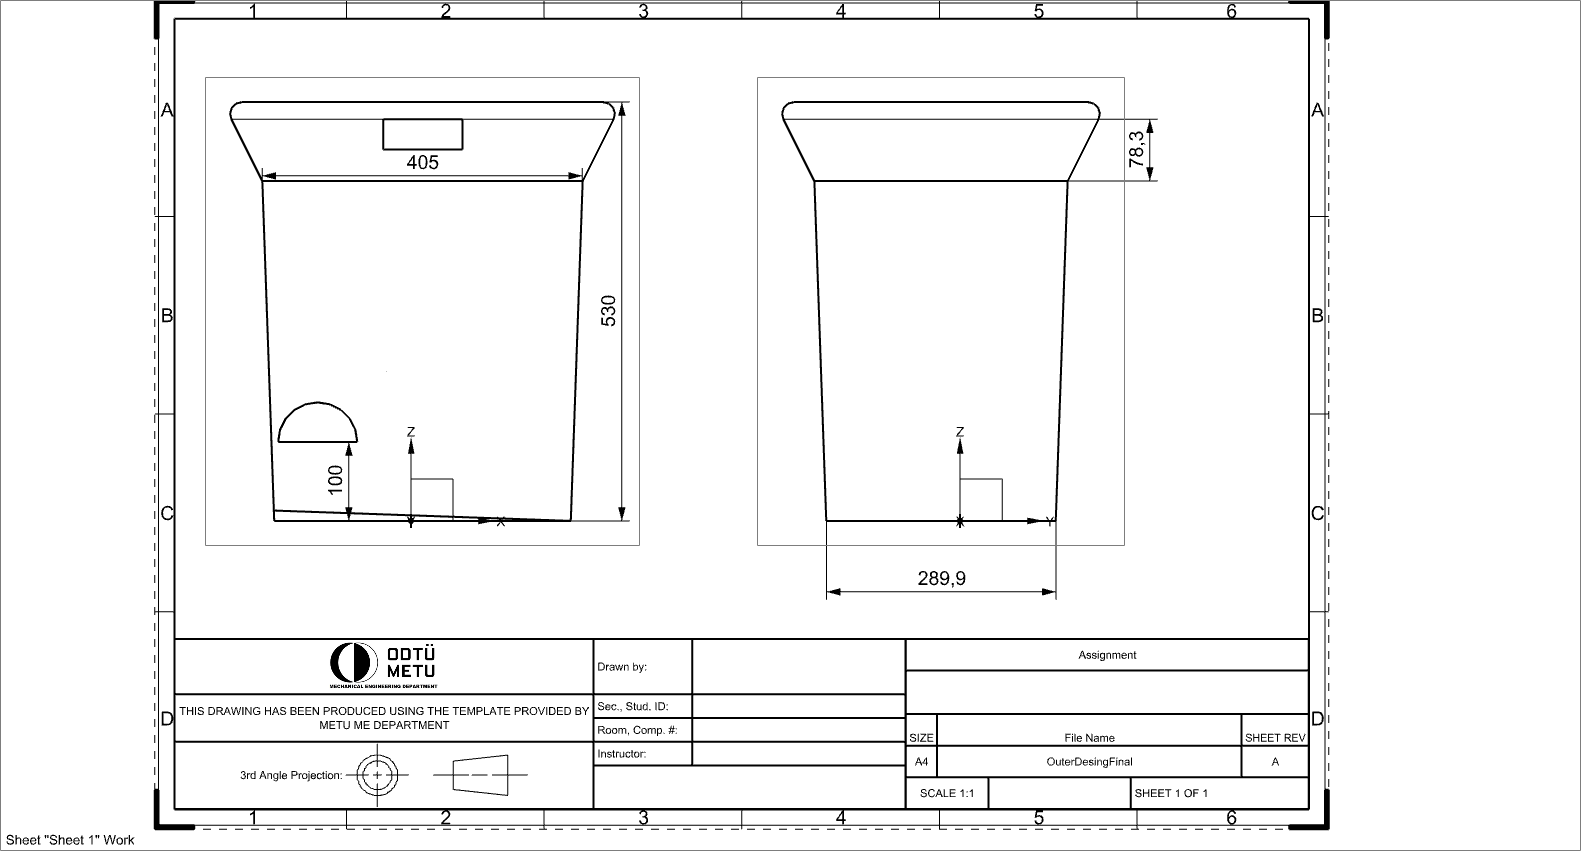
\includegraphics[width=\linewidth]{content/060_mechanical_design/5Technical.png}
     \end{subfigure}
     \caption{The Technical Drawing of the Outer Design}
     \label{fig:OuterBox}
\end{figure}

From the figures, it can be seen that there exists a handle at the upper side for lifting. In addition to that, the half circle is being cut in order for food to flow out. This is the place where food will leave the box. 

Interior design is mainly the design of the inner box. Inner box is composed of three sub-parts namely:

\begin{itemize}
    \item Connection of electronic equipment.
    \item Food mechanism.
    \item Camera unit.
\end{itemize}

\subsubsection{Connection between electronic devices}
The unplanned connection between the electronic components results with a messy looked box, therefore the inner connections are arranged such that one can easily see the connections and reach the problematic area when there is an issue. In order to satisfy this condition, the electronic devices that will be work together are grouped and put together on the solid surface. When there exists a problem in one specific sub-unit, the technician can reach that specific location and fix the problem easily. The board design can be seen on Fig~\ref{fig:Board}. The details of the electronic components can be found in electronics part of this report.
\begin{figure}[ht] 
     \centering
     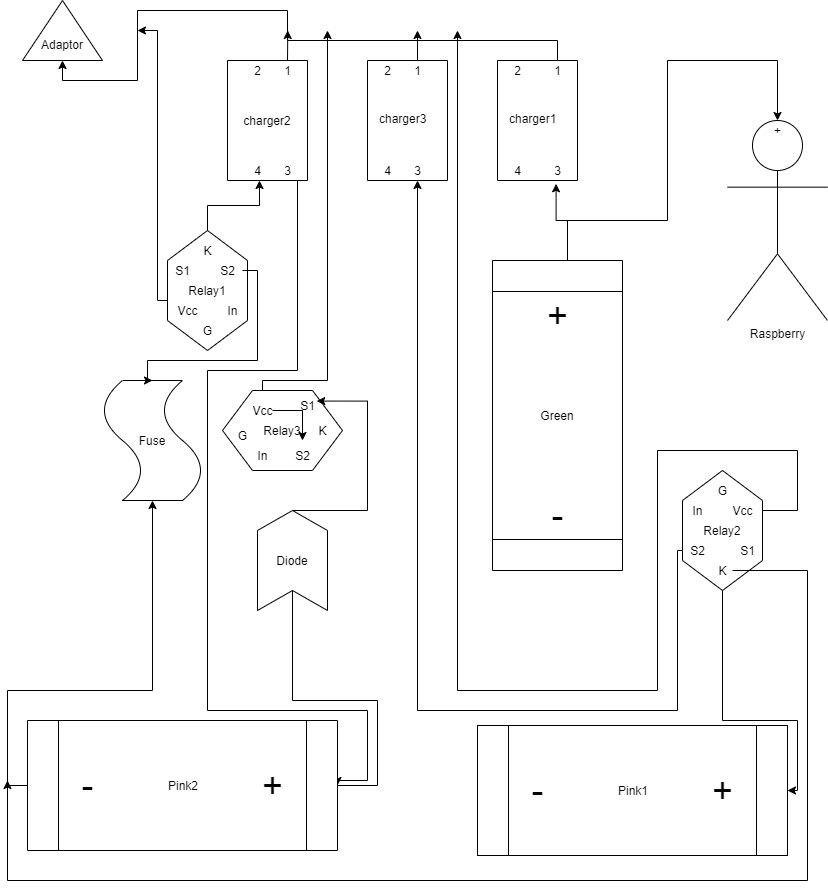
\includegraphics[width=0.9\linewidth]{content/060_mechanical_design/ElectronicBoardDesign.png}
     \caption{Electronic Board Design}
     \label{fig:Board}
\end{figure}
\clearpage 
\subsubsection{Food Mechanism}
Food mechanism is designed such that it will provide minimum 100 meals of food for an ordinary cat and the food flow should be controllable. 

An ordinary cat which weight 4 kg is advised to eat 60 gr of food per day \cite{cite:catfood}, assuming that cat eats twice in a day, for one meal the amount is 30 gr. Therefore the food reservoir should sustain:
\begin{equation}
    100 x 30 = 3000gr=3kg food 
\end{equation} 
Our engineers had selected food reservoir as 5 liter, that can sustain 4 kg of food at full capacity. 

The main objectives of the food mechanism is to control the given food amount, to satisfy this condition a gate is designed. The below figures represents the gate.
%satır 31 imiş burası değil

%TODO:
\begin{figure}[ht] 
     \centering
     \begin{subfigure}[b]{0.49\linewidth}
     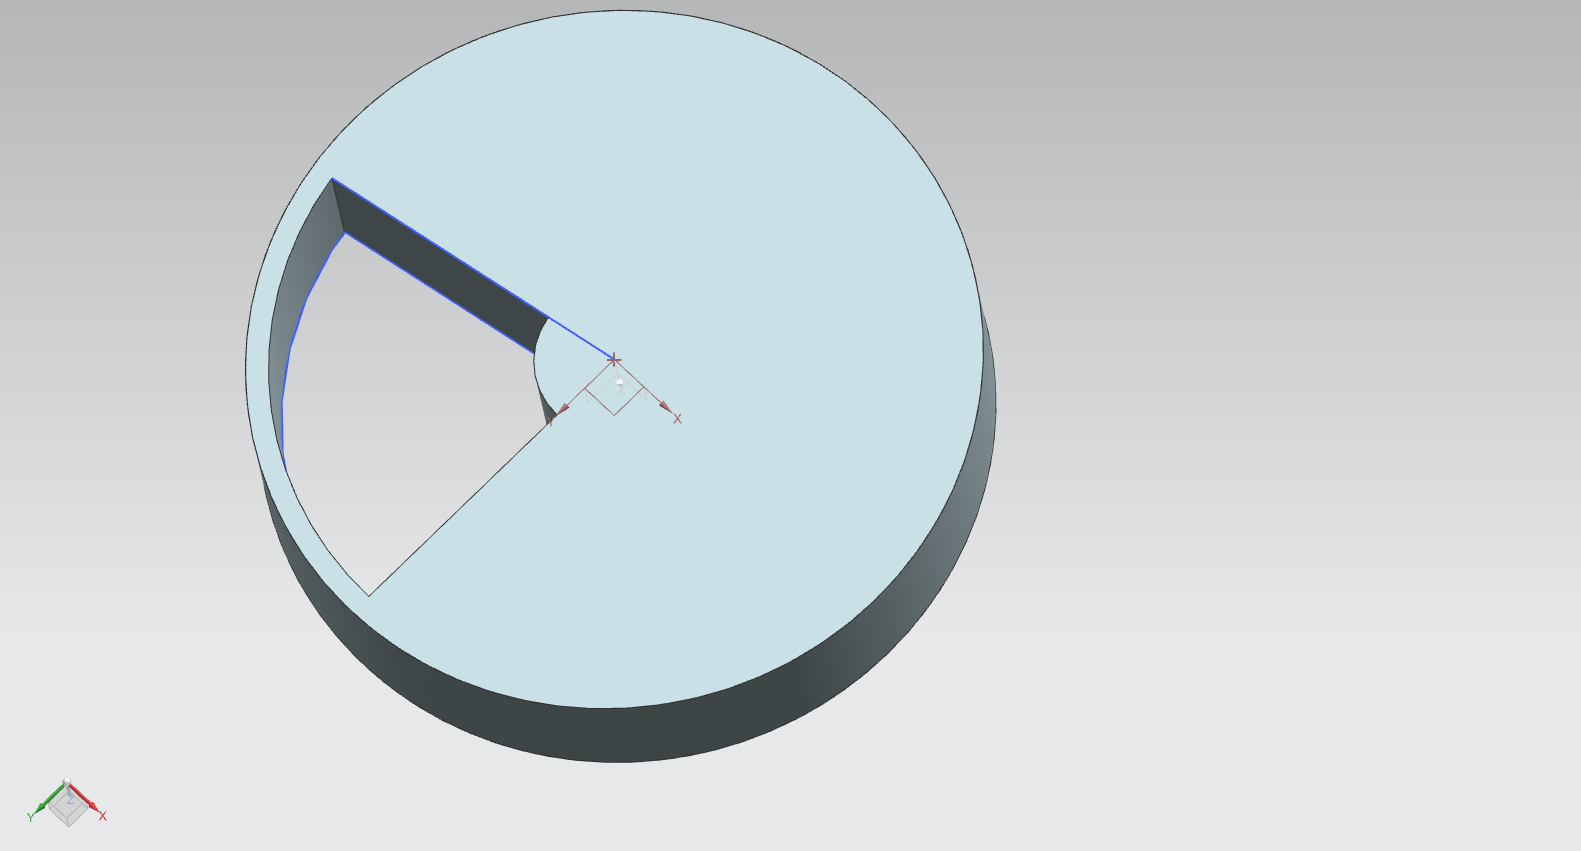
\includegraphics[width=\linewidth]{content/060_mechanical_design/cylinder.png}
     \caption{Cylinder}
     \label{fig:Cylinder1}
     \end{subfigure}
     \begin{subfigure}[b]{0.49\linewidth}
     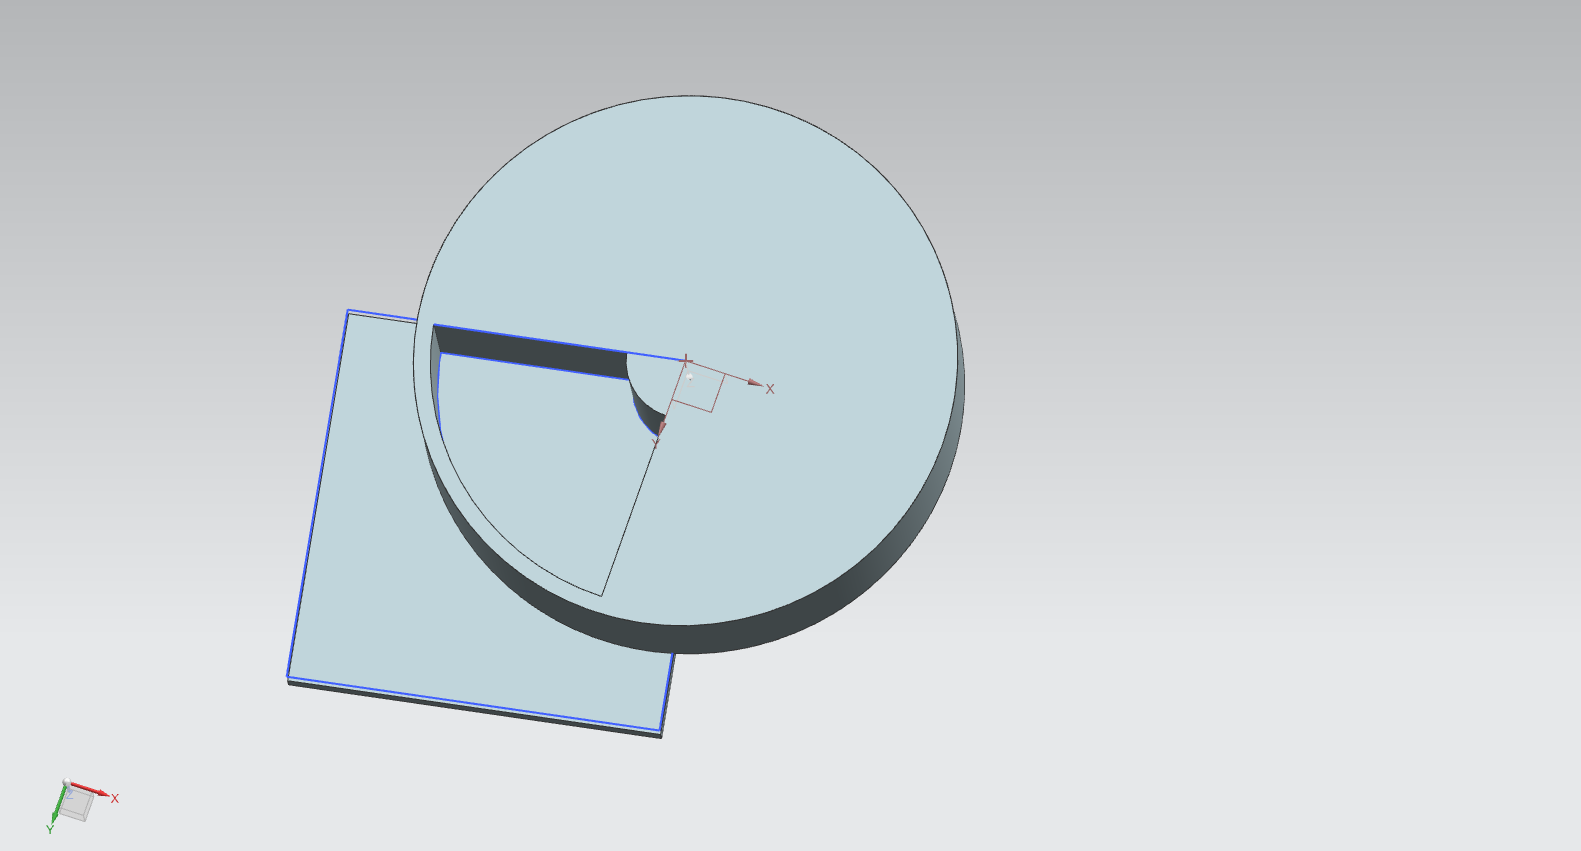
\includegraphics[width=\linewidth]{content/060_mechanical_design/cylinder2.png}
     \caption {Cylinder in Off state}
     \label{fig:Cylinder2}
     \end{subfigure}
     \label{fig:pwm}
     \begin{subfigure}[c]{0.49\linewidth}
     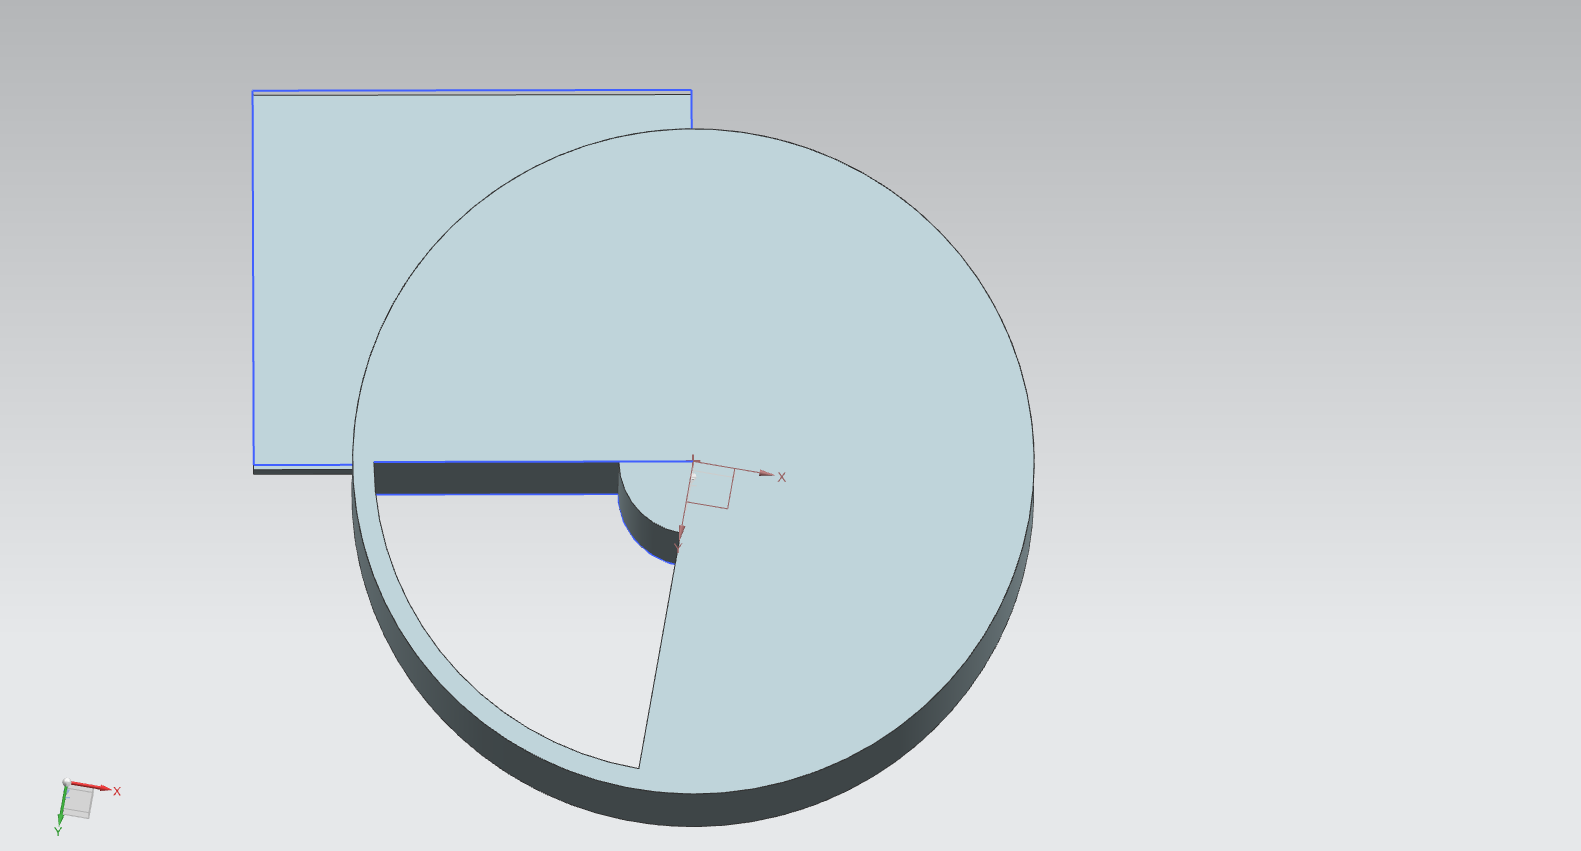
\includegraphics[width=\linewidth]{content/060_mechanical_design/cylinder3.png}
     \caption {Cylinder in On state}
     \label{fig:Cylinder3}
     \end{subfigure}
     \caption{The representation of the disk}
     \label{fig:cylinder}
\end{figure}

The Fig~\ref{fig:cylinder} represents the states of the food mechanism. Food reservoir will be placed 1 cm upward of the cylinder shown in the Fig~\ref{fig:cylinder}. Food reservoir's bottom will also be cut just like cylinder. By arranging the placement of the empty regions of cylinder and food reservoir one will change the status of the food mechanism.
The gate has two states namely OFF and ON State. In the ON state food is given whereas in the OFF state food flow is stopped. When the state is OFF the empty side of the reservoir coincides with the empty side of the cylinder and food will stop the emptiness between the reservoir and cylinder (Fig~\ref{fig:Cylinder2}). Since there exists a blockage on under the cylinder, the food will not flow downward but it will be contaminated in the reserved area. The food flow toward the empty region will continue until it is fully filled. 

The On state corresponds to the food given to the cat. When a cat arrives the servo motor rotates the cylinder shown in Fig~\ref{fig:Cylinder3}, then the empty side of the cylinder becomes free from the blockage of the barrier under it. In this way, the quantized food inside the reserved area will be given to the cat. While the reserved food is pouring the food path, the filled region of the cylinder will block the food flow from the reservoir to the cylinder, by this way only a quantized amount of food will be given to the cat at each cycle. The test results for this design can be seen at the Tests and Results, Future Test Plans part of Mechanical Design part of this report.

\begin{figure}[ht]
     \centering
     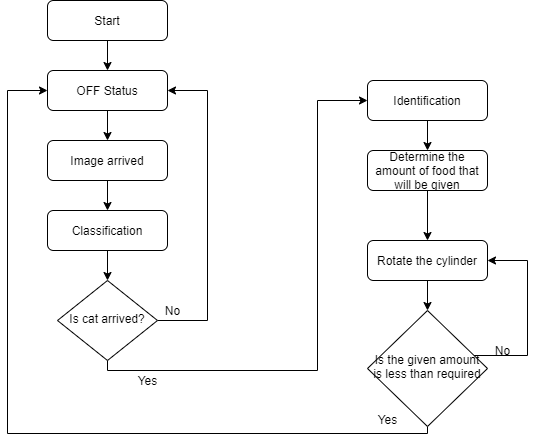
\includegraphics[width=0.8\linewidth]{content/060_mechanical_design/FoodFlowChart.png}
     \caption{Working principle of Food Mechanism}
     \label{fig:Food Flow Mechanism}
\end{figure}

In the Fig~\ref{fig:Food Flow Mechanism}  one can observe the flow chart that represents the operation principle of the Food mechanism. Our mechanism is capable of feeding at the required amounts. By processing the incoming image, the food amount that should be given will be determined. The food will be given according to the amount determined by the identification of the cat. At each cycle of rotation, the same amount of food will be given, therefore by rotating the food mechanism at the necessary amount, one can control the given food amount.  

\subsection{Requirements}

Mechanical part of the project should satisfy necessary conditions, which will be mentioned below

\begin{itemize}
    \item Total system should be lifted by an ordinary person. 
    \item Volume of the box should be enough for all electronic devices to fit in.
    \item Box should be durable for harsh outdoor conditions.
    \item Food reservoir should be provide at least 100 meals for an ordinary cat.
    \item There should be maximum \%5 waste of food. 
    \item Amount of food remaining, battery chargers while loading and in operation should be visible.
    \item Angle and the position of the camera must be adjusted properly in order to identify cats and dogs from 1.5 meter.
    \item There must be no obstacle in front of the camera unit, so that it can capture accurate photographs.
    \item Camera unit should be adjusted properly so that it should be protected from animal attacks.
\end{itemize}

\subsection{Tests and Results, Future Test Plans}
Both inner and outer designs will be tested in order to check the systems capability. The test procedures and results can be seen below.

\subsubsection{Food Mechanism}
\paragraph{Description of the Test for Food Mechanism}
Test was conducted in order to observe the behaviour of the food flow.
The purpose of this test is:
\begin{itemize}
    \item Determine the quantity of the average amount of the food poured. 
    \item Determine if there any food is jammed between reservoir and the cylinder. If there exist some, determine if they will harm to rotation or not.
    \item Determine if motor is capable of rotating without difficulty.
\end{itemize}

Procedure can be followed below.
\begin{itemize}
    \item Fully fill the reservoir with food.
    \item Observe the food flow in reservoir in off condition.
    \item Rotate the cylinder and observe the amount of food flow.
    \item While rotating observe the food flow from reservoir to the solid part of the cylinder. Observe if food is flowed from the solid part of the cylinder.
    \item Observe if there exist any food jammed between the solid part of the cylinder and the reservoir. 
    \item Return the cylinder to its old position.
    \item Observe if the flow of the food is completely stopped. 
    \item Turn the cylinder again and observe the food flow again. Compare with the previous amount of food flowed.
    \item Repeat this process until reservoir is fully empty.
\end{itemize}

The expected quantitative test results from the test is:
\begin{itemize}
    \item Food should flow through the inside of the empty region of the cylinder only. There shouldn't be any food flowing out of the cylinder. 
    \item The cylinder should completely cut the food flow from reservoir when system is in ON state.
    \item The jamming between cylinder and reservoir is expected however, the motor should be able to rotate the cylinder without any difficulty.
\end{itemize}

\paragraph{Test Results for Food Mechanism}
The test mentioned above is conducted and results can be seen below.

\begin{itemize}
    \item It is observed that the average poured food per rotation is 18 gr.
    \item Although food is jammed between the reservoir and cylinder, it did not affect the performance of the overall system. The rotation continued without any difficulty. 
    \item The jammed food also poured out of the box at following rotations, therefore it is observed that there can be an underestimation on the amount of the food given if one only considers the poured food is only due to the food that was stored in the cylinder. However, the amount of the food poured which was the resultant of the jammed food is \%7 on average of the total poured food.
    \item The variation on the amount of the food flow between rotations did not differ much. At maximum case, the amount of the food flow is 60 gr. Generally, the mass of the poured food is between 10 gr to 20 gr. 
    \item At 86 rotations the poured food is between 10 gr to 20 gr. 
    \item At 13 rotations the poured food is between is less than 10 gr but not zero.
    \item At 18 rotations the poured food is between 20 gr to 60 gr. 
    \item The food flow is completely stopped when system is in OFF state.
    \item It is observed that when system switches from the ON state to OFF state, there exist an undesirable food flow resulting from the previously jammed food.
    \item It is observed that the food in the reservoir is not homogeneously poured but the food at the open side of the reservoir finishes more quickly. This creates a mountain-shaped distribution which results in an accumulation of food at one side in the reservoir.    
\end{itemize}
The following bar graph (Figure~\ref{fig:FoodPoured}) shows the amounts of the food poured.
\begin{figure}[ht]
     \centering
     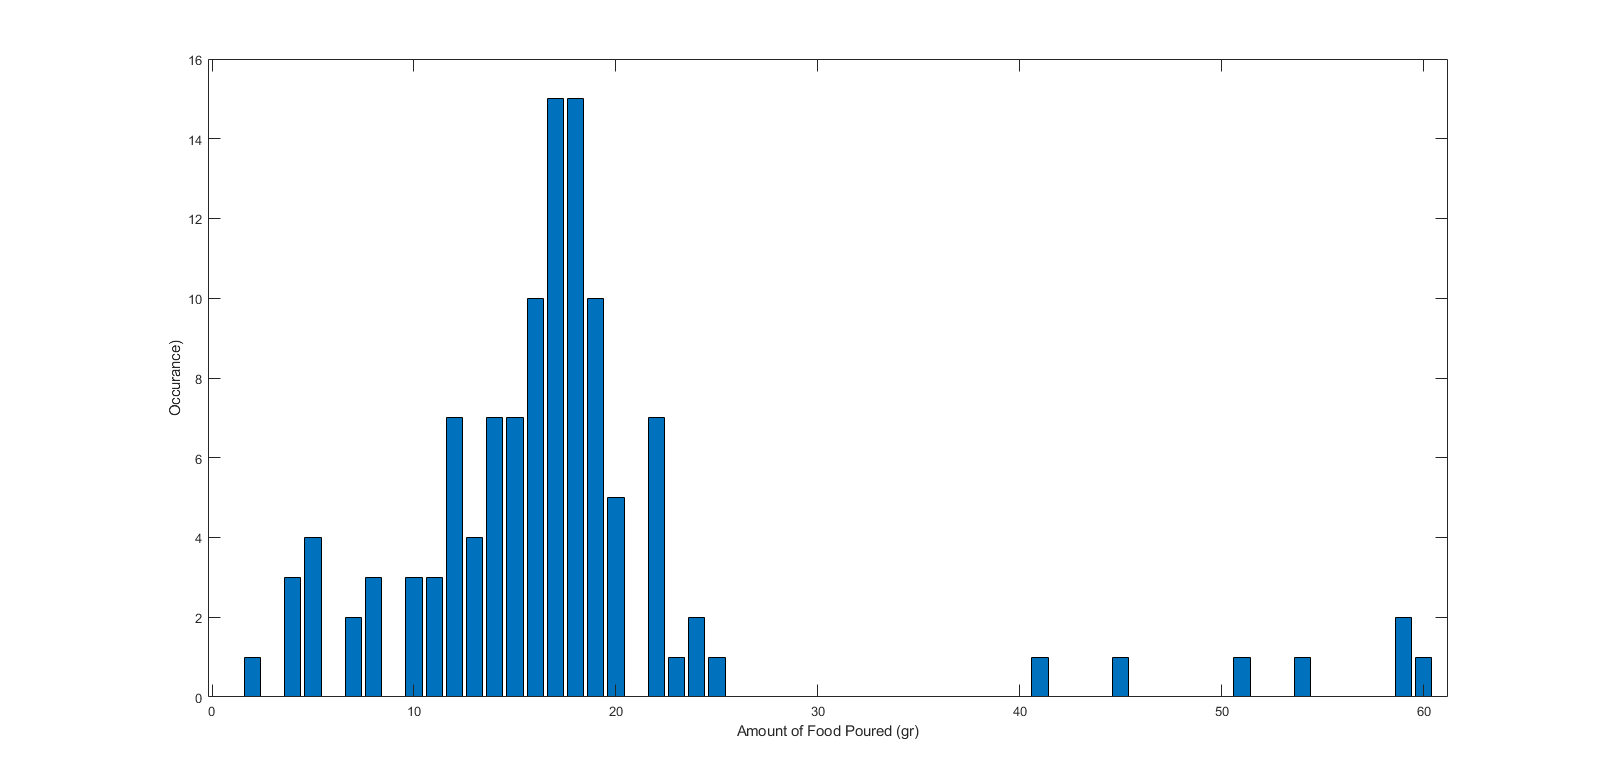
\includegraphics[width=\linewidth]{content/060_mechanical_design/FoodPoured.png}
     \caption{The Amount of Food Poured for Different Trials}
     \label{fig:FoodPoured}
\end{figure}
Where x label shows the amount of the food poured and y label shows the trial number which corresponds to that poured mount. It can be seen that graph peaks at 18-19 gr food amount and this amount can be changed by varying the rotation angle.

From previous test, which was mentioned in conceptual design report was resulted with an undesired results. According to this results the given food amount is not controllable, in addition to that there exist lots of jamming of food between reservoir and cylinder which prevented motor to turn easily. These problems are solved by rearranging the placements of cylinder and reservoir. Now they are more closely placed that jamming is minimized. In addition to that, the motor was poperly fixed to its place such that when it rotates, it does not wobble which now the food flow has become controllable. The results of the new experiment shows that food system is reliable but has some errors.

From the result of the experiment it can be said that food mechanism works properly for but there exists some errors. In two trials poured food is 59 gr which is happened at the first trials of the experiment. It shows us that system needs to be settle down before it operates properly. 

The experiment also shows that when the food amount is lowered in the reservoir, the poured food also decreases, since the food flow from the reservoir to the cylinder is not homogeneous.


\subsubsection{Exterior Design}
The purpose of the tests is to determine the reliability of the box.
\begin{itemize}
    \item Apply force on the box and check if there exist any considerable damage seen at the outside of the box. If not continue.
    \item Place electronic devices and the food mechanism inside the box and apply force on the box. Check if electronic devices, camera and food mechanism works properly. Check the angle of the camera. Observe if it works functional. Repeat this process 5 times. 
\end{itemize}

\begin{itemize}
    \item Raise the box to half a meter height and release it to the tile surface. \item Observe if there exist any considerable damage seen at the outside of the box. If not continue.
    \item Check if electronic devices, camera and food mechanism works properly. Check the angle of the camera. Observe if it works functional. Repeat this process 5 times. 
\end{itemize}

The measure of success for this experiment is having non-considerable damage on the box and it is desired that all electronic devices and the food mechanism work properly, meaning that all electronic devices and food mechanism works as if before. Moreover, the camera can move a little but it is expected to capture photographs that is useful for identifying cats and dogs.

\subsection{Modifications}
\subsubsection{Food Mechanism}
According to the test conducted on the food mechanism, it is seen that the food given in each cycle is close to each other. It is reliable, however there exist an undesired situations such as the food flow between the switching states. In order to solve this problem, first the food squeze between reservoir and cylinder should be minimized. Therefore more careful placement of the cylinder is required. In addition to that adding a food path between cylinder and reservoir can solve this problem.

It is observed that food flow from the reservoir is not homogeneous, moreover the food at the non-empty side of the reservoir is not poured through the cylinder. In order to solve this problem, our engineers will develop a ramp which will force food to flow through the empty region of the reservoir.

Test results show that, in first two or three trials after food is placed into the reservoir system poured more than expected. To solve this problem another food path will be developed and will be placed inside the reservoir, which will homogeneously fill the reservoir. By this way the first poured food into reservoir will not directly stuck in between food mechanism and reservoir but it will be placed into the empty region in Fig~\ref{fig:cylinder}.

\subsection{Compatibility Analysis of Mechanics}
It is observed that the food system is reliable when it works alone, but what if all circuit operates together. Previous tests showed that Raspberry Pi zero creates a soft pwm that suffers from glitches when the camera unit and food mechanism operates together. Therefore, in order to drive food mechanism, another microcontroller will be used and its pwm can be seen in Fig~\ref{fig:pwmaaa} in the electronics of this report

In addition to that, food system is reliable in terms of the amount of the poured food. In each cycle the poured food is similar. The servo motor did not face any hard time while rotating the cylinder although there is a jamming between reservoir and cylinder. The torque of the servo motor is capable for this project.